\documentclass[11pt,a4paper]{report}
\usepackage[utf8]{inputenc}
\usepackage{amsmath}
\usepackage{graphicx}
\usepackage{gensymb}
\usepackage{tikz}
\usepackage{pgfplots}
\usepackage{mathtools}
\usepackage{minted}
\usetikzlibrary{arrows,positioning}
\tikzset{
  %Define standard arrow tip
  >=stealth',
  % Define arrow style
  pil/.style={
      ->,
      thick,
      shorten <=2pt,
      shorten >=2pt,}
}
\usepackage{geometry}
\geometry{
  left=2cm,
  right=0.64cm,
  top=0.64cm,
  bottom=2cm
}
\usepackage{multicol}
\setlength{\columnsep}{1cm}
\graphicspath{ {images/} }

\begin{document}

\chapter{Semester 2 Examination 2013-2014\\CZ4013 Distributed System}

\begin{multicols*}{2}

\section{Question 1}

\noindent \textbf{Question 1a}

\noindent In at-least-once invocation semantics, if a client receives a reply message, the request has been executed for one or more than one times at the server. In at-most-once invocation semantics, if a client receives a reply message, the request has been executed for exactly one time. 

\noindent In at-least-once invocation semantics, when server receive a duplicate request, it will re-execute the request. In at-most-once invocation semantics, when server receive a duplicate request, it will send the previous reply again to the client.\\

\noindent \textbf{Question 1b}

\noindent Information given in the question:
\begin{itemize}
  \item Time spent in critical section by any process: $c$
  \item Message transmission delay: $d$
  \item Number of processes: $n$
\end{itemize}

\noindent For any algorithm, maximum throughput happens when when every process constantly wants to enter a critical section.\\

\noindent For central server algorithm, the throughput is:
$$\text{throughput}=\frac{1}{2d + c}$$

\noindent For ring-based algorithm, the throughput is:
$$\text{throughput}=\frac{1}{d + c}$$

\noindent For Ricart-and-Agrawala algorithm, the throughput is:
$$\text{throughput}=\frac{1}{d + c}$$

\noindent \textbf{Question 1c i}

\noindent When the freshness interval is 3 seconds, the client will only read the local cache within 3 seconds after the last validation time. If current time has passed 3 second freshness interval, the client will validation the file again with the server.\\

\noindent Take note that NFS server operations are stateless and idempotent.\\

\noindent Here is a list of consequences of client $A$ operations:
\begin{enumerate}
  \item $r_1$: Since the cache is empty, client contacts server to get latest file. Client read the local copy, which is \emph{not} the most recent update by $B$.
  \item $r_2$: Client reads local copy of the file, which is \emph{not} the most recent update by $B$.
  \item $r_3$: Since the file is not fresh, client contacts server to validate the file. Since the file has been updated by $B$, server transfer the latest file to client. Client then read the most recent update of the file. 
  \item $r_4$: Client read the local copy, which is \emph{not} the most recent update by $B$.
  \item $r_5$: Since the file is not fresh, client contacts server to validate the file. Since the file has been updated by $B$, server transfer the latest file to client. Client then read the most recent update of the file. 
  \item $r_6$: Client read the local copy, which is \emph{not} the most recent update by $B$.
  \item $r_7$: Since the file is not fresh, client contacts server to validate the file. Since the file has been updated by $B$, server transfer the latest file to client. Client then read the most recent update of the file. 
  \item $r_8$: Client read the local copy, which is the most recent update by $B$.
\end{enumerate}

\noindent The time points when $A$ needs to contact the server are $r_1,r_3,r_5,r_7$.\\

\noindent The read operations of $A$ that return the most recent update by $B$ are $r_3,r_5,r_7,r_8$. \\

\noindent \textbf{Question 1c ii}

\noindent Callback mechanism is used to maintain cache con- sistency of client side. However, if there is an update at server side before a client close a session / file, the callback has no effect on the file at currect session. \\

\noindent As a result, only the read operation at $r_6,r_7,r_8$ read the most recent update by $B$. \\

\noindent The time points when $A$ needs to contact the server are $r_1,r_6$.\\

\section{Question 2}

\noindent \textbf{Question 2a}

\begin{minted}{Java}
// StockNotification.java
public interface StockNotification 
    implements Remote {
  public void register(Callback cbObject, 
      int percentage) 
      throws RemoteException;
  public void deregister(Callback cbObject) 
      throws RemoteException;
}

// Callback.java
public interface Callback 
    implement Remote {
  public void stockAlert(String companyName) 
      throws RemoteException;
}
\end{minted}

\noindent \textbf{Question 2b i}

\noindent All possibility of $c$ and $c$:

\begin{center}
\begin{tabular}{|c|c|}
  \hline
  $c$ & $d$ \\
  \hline
  0  & 0  \\
  0  & 2  \\
  0  & 12 \\
  2  & 2  \\
  2  & 12 \\
  12 & 12 \\ \hline
\end{tabular}
\end{center}

\noindent \textbf{Question 2b ii}

\noindent Monotonic-read: If a client reads the value of a data object x, any successive read operation on x by that client will always return that same value or a more recent value.\\

\noindent If $c=10$, then it means that the $write(x\leftarrow x + 2)$ has not been propagated to the replica where $write(x\leftarrow x + 10)$ was performed. So when the same client read the value again, the value could be the currect value $10$, or a more updated value $12$.

\noindent \textbf{Question 2b iii}

\noindent Read-your-write: The effect of a write operation by a client on a data object $x$ will always be seen by a successive read operation on $x$ by the same client.\\

\noindent $a$ must be equal to 2 and $b$ must be equal to 12.\\


\noindent \textbf{Question 2b iv}

\noindent Write-follow-reads: A write operation by a client on a data object $x$ following a previous read operation on $x$ by the same client is guaranteed to take place on the same or a more recent value of $x$ that was read.\\

\noindent $d$ can be 0, 2, or, 12.

\section{Question 3}

\noindent \textbf{Question 3a i}

\noindent In routing, each node $n$ sends a query for key $k$ to the node in entry $\lfloor log_2(k-n) \rfloor + 1$. To route from N76 to $K58 \equiv 58 + 128 = K186$, we use the:

$$\lfloor log_2(186-76) \rfloor + 1 = 7\text{-th entry}$$

\noindent The 7th entry of N76 is:

$$76 + 2^{7-1} = 140 \equiv \text{N13}$$

\noindent Now, we are at N13. To route from N13 to K58, we use the:

$$\lfloor log_2(58-13) \rfloor + 1 = 6\text{-th entry}$$

\noindent The 6th entry of N13 is:

$$13 + 2^{6-1} = 45 \equiv \text{N46}$$

\noindent Now, we are at N46. To route from N46 to K58, we use the:

$$\lfloor log_2(58-46) \rfloor + 1 = 4\text{-th entry}$$

\noindent The 4th entry of N46 is:

$$46 + 2^{4-1} = 54 \equiv \text{N55}$$

\noindent Now, we are at N55. To route from N55 to K58, we use the:

$$\lfloor log_2(58-55) \rfloor + 1 = 2\text{-nd entry}$$

\noindent The 2nd entry of N55 is:

$$55 + 2^{2-1} = 57 \equiv \text{N61}$$

\noindent Now, we are at N61, which contains the information of K58. \\

\noindent In summary, the route from N76 to K58 is N13 $\rightarrow$ N46 $\rightarrow$ N55 $\rightarrow$ N61.\\

\noindent \textbf{Question 3a ii}

\noindent The finger table for N55:

\begin{center}
\begin{tabular}{|c|c|c|c|}
  \hline
  Entry & At-least & Identifier & Range\\ \hline
  1     & 56       & N61        & $56\le x <61$\\
  2     & 57       & N61        & $57\le x <61$\\
  3     & 59       & N61        & $59\le x <61$\\
  4     & 63       & N76        & $63\le x <76$\\
  5     & 71       & N76        & $71\le x <76$\\
  6     & 87       & N116       & $87\le x <116$\\
  7     & 119      & N122       & $119\le x <122$\\ \hline
\end{tabular}
\end{center}

\noindent Let $x$ be the range of possible node identifiers of new node. By combining all the ranges, the possible value of $x$ are:
$$56\le x <61, 63\le x <76,87\le x <116,119\le x <122$$

\noindent \textbf{Question 3b i}

\noindent There is only one possibility, i.e. when both events occurs at process $p_1$. \\

\noindent \textbf{Question 3b ii}

\noindent $e_A$ occurs in process $p_2$, and $e_B$ occurs in process $p_3$.

\begin{center}
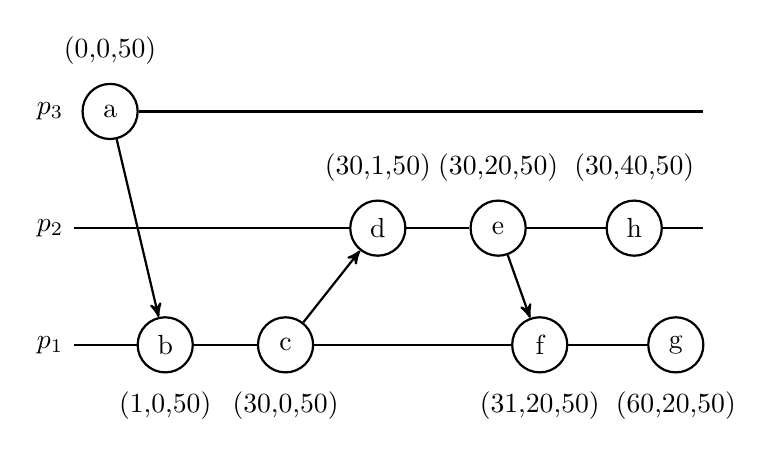
\begin{tikzpicture}[>=stealth',thick,
roundnode/.style={circle, draw=black, thick, minimum size=0.7cm},
]
\node[] (p1) {$p_3$};
\node[below=1cm of p1] (p2) {$p_2$};
\node[below=1cm of p2] (p3) {$p_1$};

\node[roundnode](a)[right = 1mm of p1.east]{a};
\node[roundnode](b)[right = 8mm of p3.east]{b};
\node[roundnode](c)[right = 8mm of b]{c};
\node[roundnode](d)[right = 35mm of p2.east]{d};
\node[roundnode](e)[right = 8mm of d]{e};
\node[roundnode](f)[right = 25mm of c]{f};
\node[roundnode](g)[right = 10mm of f]{g};
\node[roundnode](h)[right = 10mm of e]{h};

\node[right = 80mm of p1](d1){};
\node[right = 80mm of p2](d2){};
\node[right = 80mm of p3](d3){};

\draw[->] (a) -- (b);
\draw[-] (b) -- (c);
\draw[->] (c) -- (d);
\draw[-] (d) -- (e);
\draw[-] (e) -- (h);
\draw[->] (e) -- (f);
\draw[-] (f) -- (g);

% Dummy 
\draw[-] (p2) -- (d);
\draw[-] (p3) -- (b);
\draw[-] (a) -- (d1);
\draw[-] (h) -- (d2);
\draw[-] (g) -- (d3);
\draw[-] (c) -- (f);

% Label
\node[above=1mm of a](labela){(0,0,50)};
\node[below=1mm of b](labelc){(1,0,50)};
\node[below=1mm of c](labelc){(30,0,50)};
\node[above=1mm of d](labeld){(30,1,50)};
\node[above=1mm of e](labele){(30,20,50)};
\node[below=1mm of f](labelf){(31,20,50)};
\node[below=1mm of g](labelg){(60,20,50)};
\node[above=1mm of h](labelg){(30,40,50)};

\end{tikzpicture}
\end{center}

\section{Question 4}

\noindent \textbf{Question 4a}

\noindent Since we know $t_g$ and $t_e$ and some intervals, we can know all the time at all events. To synchronize $p_3$ clock with $p_2$ clock, $p_3$ sets its clock to:

$$t_g - (t_h - t_g)$$

\noindent The accuracy is 100\% \\

\noindent \textbf{Question 4b}

\noindent To synchronize $p_3$ clock with $p_1$ clock, $p_3$ sets its clock to:

$$t_e + (t_f - t_e) + 400 + (t_h - t_g)$$

\noindent The accuracy is 100\% \\

\noindent \textbf{Question 4c}

\noindent [Help wanted!]\\

\noindent \textbf{Question 4d}

\noindent Possible snapshots are:

\begin{itemize}
  \item $S_d, S_c, S_a$
  \item $S_e, S_c, S_a,e\rightarrow f$
  \item $S_e, S_f, S_a$
  \item $S_e, S_g, S_a,g\rightarrow h$
  \item $S_e, S_g, S_h$
\end{itemize}

\end{multicols*}
\end{document}
